% AETHER-2.5D Studio — IEEE-style paper (IEEEtran). Generated from docs/paper/src/content.mjs.
% Compile: pdflatex aether_ieee.tex (twice), or upload docs/paper/ to Overleaf.
% Copyright (c) 2026 Rachel (AiChan277). Licensed under the AETHER-2.5D Studio Source-Available,
% No-Derivatives, No-AI License v1.0 (see LICENSE). Not for AI training or reproduction.
\documentclass[conference]{IEEEtran}
\IEEEoverridecommandlockouts
\usepackage[utf8]{inputenc}
\usepackage[T1]{fontenc}
\usepackage{textcomp}
\usepackage{amsmath,amssymb,amsfonts}
\usepackage{graphicx}
\usepackage{cite}
\usepackage{url}
\usepackage{xcolor}
\def\UrlBreaks{\do\/\do-\do.\do_}
\def\BibTeX{{\rm B\kern-.05em{\sc i\kern-.025em b}\kern-.08em T\kern-.1667em\lower.7ex\hbox{E}\kern-.125emX}}

\begin{document}

\title{AETHER-2.5D Studio: A Real-Time, Multi-Backend 2.5D Non-Photorealistic Rendering and NPU-Accelerated Tracking Engine for Virtual Performers}
\author{\IEEEauthorblockN{Rachel}
\IEEEauthorblockA{\textit{DSD-Aether Project}\\
Email: \url{ramzyhaidar20@gmail.com}}}
\maketitle

\begin{abstract}
Virtual performers (``VTubers'') need an avatar that follows the body in real time, looks like a hand-drawn 2D illustration rather than a shaded 3D model, and reaches streaming software with a transparent background and minimal latency, all on hardware that ranges from integrated laptop GPUs to high-end discrete cards. This paper describes AETHER-2.5D Studio, a Windows desktop engine built to a single technical specification that meets these goals. A neural tracking stage runs Google MediaPipe models through ONNX Runtime with a six-tier execution-provider router that prefers the Intel AI Boost neural processing unit (NPU), and enforces a C$^1$-continuous hyperbolic-tangent movement boundary and an iterative capsule anti-clipping projection \textit{before} poses reach a 240 Hz animation solver. A ``2.5D'' renderer then drives a VRM avatar through a 14-pass frame graph implemented on Vulkan 1.3, DirectX 12 with DirectX Raytracing (DXR) 1.1, and DirectX 11, under a unified coordinate contract that makes the DirectX 12 output pixel-identical to Vulkan. Lighting scales across three tiers (rasterized traditional toon lighting, hybrid ray-traced shadows, and a temporally locked stylized path tracer), and one-bounce indirect light is folded into the cel quantizer's input so that colour bleeding never reintroduces 3D gradients. The system adds a dynamic Kajiya-Kay ``angel ring'', a depth-offset rim light, an edge-preserving Kuwahara and difference-of-Gaussians illustration filter, and a circadian lighting model. Measured on an RTX 5060 laptop GPU with an Intel NPU, the ray-traced 1080p critical path takes 2.67 ms at the 95th percentile, NPU face tracking 3.35 ms, end-to-end motion-to-photon 8.33 ms, and DirectX 12 matches Vulkan with a silhouette intersection-over-union of 1.000.
\end{abstract}

\begin{IEEEkeywords}
Non-photorealistic rendering, toon shading, real-time ray tracing, path tracing, spatiotemporal filtering, DirectX 12, Vulkan, neural processing unit, pose estimation, virtual avatars, VTuber, lock-free concurrency
\end{IEEEkeywords}


\section{Introduction}
Live streaming with an animated avatar instead of a camera image has become a mainstream form of entertainment. The performer's face, body, and hands are captured by a webcam, the motion is retargeted onto a character, and the rendered character is composited into a broadcast. Two artistic traditions dominate: \textit{Live2D} rigs~\cite{live2d}, which deform layered 2D artwork and therefore look exactly like an anime illustration but cannot turn far from the drawn viewpoint, and 3D models in formats such as VRM~\cite{vrm}, which can move freely but usually look like a game character rather than a drawing.

AETHER-2.5D Studio aims to deliver both: real 3D freedom of motion with an image that reads as flat, hand-painted 2D art. We call this \textit{2.5D}. The engine is written in C++20 and Rust, targets Windows 10 and 11 on x86-64, and was implemented in six verified phases against a binding internal specification (AETHER-TS-001). This paper describes the complete system literally, as built, together with the measurements that its automated test suite records.

Three practical constraints shaped the design. First, latency: the avatar must react within one display frame of the performer, which rules out locks and heap allocation on every real-time thread. Second, hardware diversity: many performers stream from laptops with integrated GPUs, while others own GPUs with hardware ray tracing, so the same project must scale from an Intel iGPU to an RTX-class card and across graphics APIs. Third, art direction: physically based effects such as soft shadows and global illumination are desirable only if they do not destroy the flat, crisp look of cel animation.

The contributions of this work are:

\begin{itemize}
\item a lock-free, allocation-free five-thread architecture with a frozen 64-byte-aligned C/Rust foreign-function interface (Section III);
\item an NPU-first tracking pipeline whose post-processing enforces a C$^1$-continuous $\tanh$ movement boundary and zero-penetration capsule anti-clipping at the tensor level (Section IV);
\item a multi-backend renderer (Vulkan 1.3, DirectX 12 with DXR 1.1, DirectX 11) with an explicit anti-flip coordinate contract and automatic hardware tiering for integrated GPUs (Sections VI-A and VI-B);
\item a three-tier lighting architecture in which ray-traced and path-traced indirect light is integrated \textit{before} cel quantization, plus dynamic anisotropic hair specular, depth-offset rim light, an illustration post-filter, and circadian lighting (Sections VI-C to VI-H);
\item a verification methodology with 30 C++ test suites that measure every claim in this paper (Sections VIII and IX).
\end{itemize}


\section{Related Work}

\subsection{Monocular Face, Body, and Hand Tracking}
MediaPipe~\cite{mediapipe} popularized on-device perception pipelines built from small, fast networks. BlazeFace~\cite{blazeface} detects faces in under a millisecond on mobile GPUs; the MediaPipe Face Mesh~\cite{facemesh} regresses 468 3D surface landmarks; BlazePose~\cite{blazepose} and MediaPipe Hands~\cite{mphands} track 33 body and 21 hand keypoints per hand. Rigid head pose can be recovered from such landmarks with orthogonal Procrustes alignment~\cite{gower}, solved in closed form by the Kabsch algorithm~\cite{kabsch}. Raw landmark streams are noisy; the 1\texteuro{} filter~\cite{oneeuro} trades jitter against lag adaptively, and Kalman filtering~\cite{kalman} adds prediction. AETHER-2.5D uses all of these established components and contributes the scheduling, hardware routing, and post-processing around them.


\subsection{Toon and Non-Photorealistic Rendering}
Early real-time toon shading quantized the diffuse term through a 1D texture~\cite{lake}, and Gooch \textit{et al.}~\cite{gooch98} introduced cool-to-warm tone shading for illustration; the field is surveyed by Gooch and Gooch~\cite{npr_book}. Silhouettes are commonly drawn by rendering back faces of an expanded mesh, a variant of the image-precision silhouette method of Raskar and Cohen~\cite{raskar}. Production anime-style 3D, most famously in \textit{Guilty Gear Xrd}~\cite{ggxrd}, relies on hand-edited normals, per-vertex shadow thresholds, and inner lines to make 3D read as 2D. The VRM ecosystem standardizes a toon material, MToon~\cite{mtoon}. Our renderer follows this tradition but replaces hand-edited face normals with a baked face shadow signed-distance field and adds physically based terms in a quantization-aware way.


\subsection{Real-Time Ray Tracing and Denoising}
The rendering equation~\cite{kajiya86} is the foundation of path tracing~\cite{pbrt}. Hardware ray tracing exposed through DirectX Raytracing~\cite{dxr} and Vulkan ray queries~\cite{vulkan} made a few rays per pixel affordable in real time, but low sample counts require reconstruction. Spatiotemporal variance-guided filtering (SVGF)~\cite{svgf} combines temporal accumulation with variance-driven à-trous filtering, and temporal anti-aliasing practice~\cite{karis} contributes neighbourhood clamping against ghosting. Self-intersection along shading normals is a well-known source of artifacts~\cite{wachter}. Soft shadows with contact hardening are commonly approximated by percentage-closer soft shadows~\cite{pcss}. Spatially blue-noise sample distributions~\cite{heitz} improve perceived quality at very low sample counts.


\subsection{Image-Space Stylization}
The Kuwahara filter~\cite{kuwahara} and its anisotropic generalization~\cite{kyprianidis} flatten regions into painterly patches while preserving edges, as the bilateral filter~\cite{tomasi} does for smoothing. Coherent line drawing~\cite{kang} and the extended difference-of-Gaussians (XDoG)~\cite{xdog} extract stylized lines from images. We apply simplified single-pass variants to an already stylized render, where their role is to remove residual 3D curvature rather than to abstract a photograph.


\subsection{Hair Shading}
Kajiya and Kay~\cite{kajiyakay} modelled hair as thin cylinders with a specular term that depends on the tangent rather than the normal. Marschner \textit{et al.}~\cite{marschner} derived physically measured primary and secondary lobes, and Scheuermann~\cite{scheuermann} showed that shifting the tangent along the normal produces two offset highlights cheaply in real time. Our ``angel ring'' applies this model and then quantizes it.


\section{System Architecture}

\subsection{Thread Topology and Lock-Free Channels}
The application runs five real-time thread classes plus background workers (Table I). Each pair of communicating threads is connected by a single-producer single-consumer ring or a lock-free triple buffer~\cite{herlihy}, so producers never block consumers and a consumer always reads the newest complete value. Two hard rules are enforced in continuous integration: no heap allocation inside any real-time tick (HR-01, checked at run time in Debug builds by a scoped allocation guard), and no mutex, condition variable, slim reader/writer lock, or critical section in the core, RHI, tracking, animation, renderer, or output modules (HR-02). Per-frame memory comes from pre-sized frame arenas, pools, and fixed-capacity vectors.

\begin{table}[!t]
\renewcommand{\arraystretch}{1.15}
\caption{Thread topology}
\label{tab:threads}
\centering\footnotesize
\begin{tabular}{p{0.188\columnwidth}p{0.254\columnwidth}p{0.498\columnwidth}}
\hline
\textbf{Thread} & \textbf{Placement} & \textbf{Role} \\
\hline
T0 Main & Normal & Win32 window, messages, device/DPI events \\
T1 Vision & Highest, MMCSS & Camera, pre-processing, ONNX inference, NPU post-processing \\
T2 Sim/IK & Highest, P-core & 240 Hz filters, IK, SpringBone, expressions \\
T3 Render & Highest, P-core & Frame graph, late-latch pose, UI \\
T4 Output & Above normal & Spout2, virtual camera, NDI, DSP sync \\
Workers & Below normal, E-cores & Logging, crash dumps, asset loading \\
\hline
\end{tabular}
\end{table}

T2 ticks at a fixed 240 Hz and whenever a new pose arrives. T3 uses a phase-locked frame timer that wakes 0.2 ms after the simulation publishes, acquires the newest skinning frame as late as possible (``late latch''), and splits GPU submission into a critical command buffer (passes 1--12, signalling a timeline semaphore) and a UI command buffer (passes 13--14). T4 waits on that timeline value, so output never waits for the UI.


\subsection{Language Boundary and FFI Contract}
Latency-critical code is C++20 (MSVC v143). The VRM/glTF loader~\cite{gltf}, project persistence, node-graph compiler and evaluator, WebAssembly plugin sandbox~\cite{wasm,wasmtime}, and network I/O are Rust 2024, linked as one static library. Every structure crossing the boundary is declared once in Rust with \texttt{\#[repr(C, align(64))]}, generated into a C header, and checked by static assertions on both sides plus a run-time layout table (HR-03). Sixty-four-byte alignment places each shared structure on its own cache line, avoiding false sharing between producer and consumer threads. Every exported Rust function runs inside \texttt{catch\_\allowbreak{}unwind}, so a panic becomes an error code instead of undefined behaviour (HR-04).


\subsection{GPU Resource Lifetime}
GPU objects cannot be destroyed while in-flight frames reference them. The engine therefore retires resources through an epoch-fenced collector: objects are tagged with the frame-timeline value at retirement and reclaimed once the GPU has passed it, a scheme related to epoch-based reclamation~\cite{fraser}. An incremental tri-colour mark-sweep~\cite{dijkstra} over the resource graph bounds the cost of each collection step. Avatar hot-swaps and backend switches route through this collector.


\section{Tracking Pipeline}

\subsection{Models and Execution-Provider Routing}
Five MediaPipe models are converted from TFLite to static-shape ONNX opset 17 in NCHW layout: the BlazeFace short-range detector ($1\times3\times128\times128$), Pose Landmarker Lite ($256\times256$), Hand Landmarker with a baked batch of two for left and right hands ($2\times3\times224\times224$), the 478-point Face Landmarker, and a 52-output ARKit blendshape network~\cite{arkit}. Static shapes are required for ahead-of-time compilation on the NPU. INT8 variants are produced by static per-channel quantization over a 500-frame synthetic calibration corpus, and the build fails if the normalized mean error grows by more than 3 \% relative to FP32. Every model file is verified against a SHA-256 digest before loading.

Inference runs through ONNX Runtime~\cite{ort} with a six-tier router: TensorRT, OpenVINO~\cite{openvino} on the NPU, OpenVINO on the iGPU, DirectML on the iGPU, DirectML on the discrete GPU, and the CPU. All input and output tensors are bound once at initialization, so the per-frame call allocates nothing. A 512-slot latency ring demotes the router to the next tier when the 120-frame window exceeds 9 ms.

Camera frames arrive from Media Foundation as NV12. An AVX2 routine converts, crops, rotates, and normalizes the face, body, and hand regions of interest directly into planar RGB tensors in 0.24 ms. Head pose is solved by weighted Procrustes alignment~\cite{gower} of the 468 canonical face vertices using the Kabsch algorithm~\cite{kabsch}, and iris landmarks yield gaze.


\subsection{NPU Safe-Zone Box}
A performer leaning toward the edge of the camera frame can push the avatar out of view, and a hard clamp makes the avatar stop abruptly, which looks robotic. AETHER-2.5D therefore passes each translation component through a soft boundary before poses leave the tracking stage. Let the box be $[b_{min}, b_{max}]$ on one axis, with centre $c$ and half-width $h$, and let $u = (x - c)/h$ be the normalized offset. With a user-set \textit{soft-wall elasticity} $k \in [0.05, 0.95]$ and linear limit $\ell = 1 - k$, the mapping is

\begin{equation}
f(u) = \begin{cases} u, & |u| \le \ell \\ \operatorname{sgn}(u)\left(\ell + k \tanh\frac{|u| - \ell}{k}\right), & |u| > \ell \end{cases}
\label{eq:tanh}
\end{equation}
and the output is $x' = c + h\,f(u)$. Both branches equal $\ell$ at $|u| = \ell$, and both have unit slope there because $\frac{d}{du}\,k\tanh\frac{u-\ell}{k} = \operatorname{sech}^2(0) = 1$, so $f$ is C$^1$-continuous: motion is exactly linear inside the box, decelerates smoothly near the wall, and $|f(u)| < \ell + k = 1$ guarantees that the avatar never leaves the box. Non-finite inputs are replaced by the box centre. Head yaw, pitch, and roll are clamped to configurable limits, and any single-frame jump larger than $65^\circ$ relative to the last accepted pose is limited to $25^\circ$, which rejects landmark glitches.


\subsection{Predictive Capsule Anti-Clipping}
When a performer touches their face or crosses their arms, landmark noise can place a hand inside the avatar's head or chest, and the spring dampers downstream would then animate the error. The tracking stage therefore represents the torso, head, and back hair as capsules~\cite{ericson} built from the current head position, and projects every hand and forearm joint out of them. For a capsule with segment $\overline{ab}$ and radius $r$, the closest point is $q = a + t(b - a)$ with $t = \mathrm{clamp}\!\left(\frac{(p-a)\cdot(b-a)}{\lVert b-a\rVert^2}, 0, 1\right)$, and a penetrating point is moved to

\begin{equation}
p' = q + (r + \epsilon)\,\frac{p - q}{\lVert p - q\rVert}
\label{eq:capsule}
\end{equation}
with a forward direction used when $p = q$. Because the capsules overlap, escaping one can enter another. The projection is therefore iterated Gauss--Seidel style, as in position-based dynamics~\cite{pbd}, for up to eight passes until no constraint is violated, and the soft-boundary envelope for limbs is applied \textit{before} projection so that compression cannot pull a corrected limb back inside the body. A residual-penetration diagnostic is reported after projection. In a sweep of 2,145 hand and forearm positions through the head, torso, and hair volumes, 1,584 positions required correction and the worst residual penetration was exactly zero.


\section{Animation}
T2 consumes poses at 240 Hz. Positions and rotations are smoothed by 1\texteuro{} filters~\cite{oneeuro}, whose cutoff frequency rises with speed,

\begin{equation}
f_c = f_{c,min} + \beta\,\lvert\dot{\hat{x}}\rvert
\label{eq:oneeuro}
\end{equation}
\begin{equation}
\alpha = \frac{1}{1 + \frac{1}{2\pi f_c T_e}}
\label{eq:oneeuro-alpha}
\end{equation}
and a six-degree-of-freedom constant-velocity Kalman predictor~\cite{kalman} compensates the remaining delay. Measured static jitter is 0.98 mm in position and $0.0086^\circ$ in rotation, with a dynamic lag of 16.67 ms (one tracking frame) at 2 Hz. A \textit{visibility-first} solver blends limbs that leave the camera's view toward procedural rest poses with a rate limit of $|dw/dt| \le 4\,\mathrm{s}^{-1}$. Limbs use analytic two-bone inverse kinematics with soft extension clamping and anatomical joint limits, and the spine and neck use FABRIK~\cite{fabrik}. Hair and clothing follow VRM SpringBones integrated with Verlet steps~\cite{jakobsen} in an eight-wide AVX2 structure-of-arrays layout against sphere and capsule colliders; a full simulation tick with 512 spring joints takes 0.052 ms. Facial blendshapes are mapped from ARKit to VRM expressions, and mouth shapes cross-fade over 60 ms between camera-derived visemes and an external audio DSP that shares a 128-byte packet through shared memory.


\section{Rendering}
Shaders are written once in Slang~\cite{slang} and compiled to SPIR-V for Vulkan and to DXIL (Shader Model 6.6) for DirectX 12. The frame graph has 14 passes: GPU skinning with sparse morph targets; acceleration-structure refit; a G-buffer pre-pass with normals, motion vectors, material IDs, and stencil masks; ray-traced or rasterized shadows and colour bleed; denoising; NPR shading; inverted-hull outlines; transparent shading; crease lines; bloom with a dual-Kawase pyramid~\cite{bjorge}; the illustration filter and display transform; viewport composition; and output encoding. A pre-pass ``Z-flattening'' step compresses depth around the head pivot toward a drawing plane; at a flatness of 0.75 the nose foreshortening metric drops from 0.576 to 0.152, a 73.6 \% reduction.

\begin{figure*}[!t]
\centering
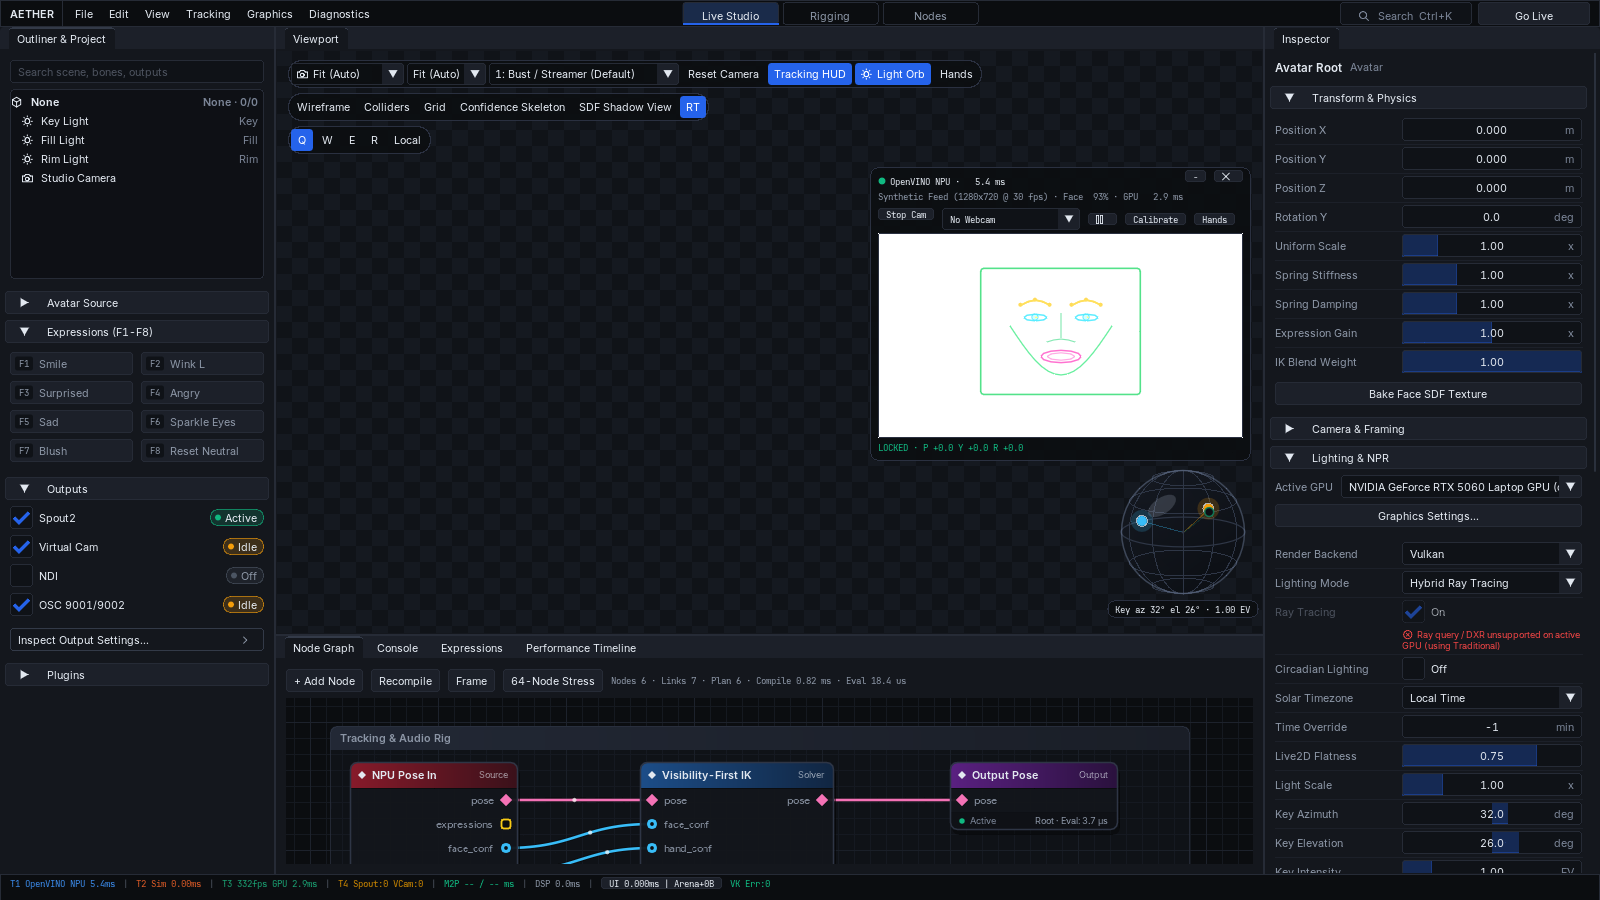
\includegraphics[width=\textwidth]{figures/fig_studio.png}
\caption{The AETHER-2.5D Studio ``Live Studio'' workspace: outliner and outputs (left), viewport with tracking HUD and light orbit control (centre), node graph (bottom), and the Inspector with Render Backend, Lighting Mode, and Circadian Lighting controls (right). Headless snapshot rendered by the test suite.}
\label{fig:studio}
\end{figure*}


\subsection{Multi-Backend RHI and the Anti-Flip Contract}
The renderer runs on Vulkan 1.3 with \texttt{VK\_\allowbreak{}KHR\_\allowbreak{}ray\_\allowbreak{}query}~\cite{vulkan}, on DirectX 12 with DXR 1.1 inline ray queries (\texttt{TraceRayInline})~\cite{dxr}, or on DirectX 11 (Shader Model 5.0) for older hardware. The backend can be switched live from the Graphics Settings menu or the Inspector. The DirectX 12 device implements command queues, triple-buffered frame fences, CBV/SRV/UAV, RTV, DSV, and sampler descriptor heaps, root signatures, graphics and compute pipeline-state objects, and acceleration structures.

Vulkan and Direct3D disagree on two conventions that silently flip images. Vulkan's clip-space $y$ axis points down and Direct3D's points up, and render targets are addressed top-left in both but sampled through different viewport transforms. A naive port therefore renders upside down, or renders upright while inverting triangle winding so that back-face culling and inverted-hull outlines turn inside out. AETHER-2.5D fixes a single contract: the projection matrix keeps one sign of $P_{11}$ for both APIs; the Direct3D viewport is given with its origin at the top-left; offscreen targets are always sampled with $v$ increasing downward, with no $1 - v$ correction anywhere in the ImGui viewport, Spout2, or virtual-camera paths; and rasterizer state declares counter-clockwise front faces on both APIs (\texttt{FrontCounterClockwise = TRUE} in \texttt{D3D12\_\allowbreak{}RASTERIZER\_\allowbreak{}DESC}). The contract is verified automatically: the test renders the same avatar with a deliberately asymmetric yaw on both APIs and compares alpha silhouettes. The DirectX 12 frame matches Vulkan with an intersection-over-union of 1.000 upright, versus 0.380 against a vertically flipped copy and 0.880 against a mirrored copy; centroids agree to three decimals, the mean RGB difference is 0.45 levels, and the D3D12 debug layer reports zero errors (Fig. 2).

\begin{figure}[!t]
\centering
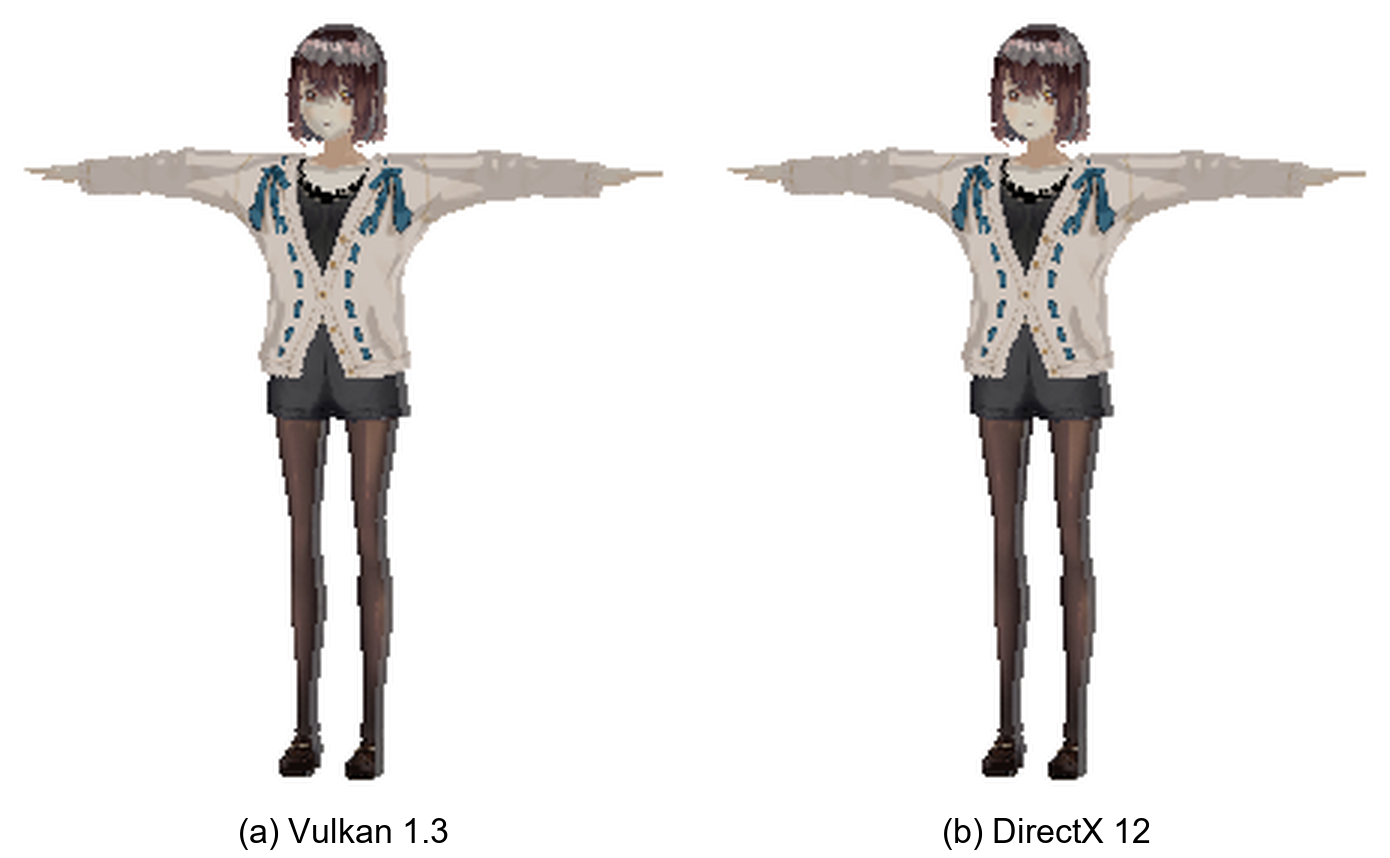
\includegraphics[width=\columnwidth]{figures/fig_parity.png}
\caption{Anti-flip verification on the VRM test avatar: (a) Vulkan and (b) DirectX 12 renders with asymmetric camera yaw. Silhouette IoU is 1.000; any vertical flip would reduce it to 0.380.}
\label{fig:parity}
\end{figure}

The DirectX 12 output reaches Spout2~\cite{spout} through D3D11On12 and a shared NT handle, and reaches the virtual camera through a readback into the same shared-memory transport that Vulkan uses. A bridge object can also hand the DirectX 12 frame to the Vulkan compositor; this path matches the standalone DirectX 12 image within 20 RGB levels.


\subsection{Integrated GPU Support and Automatic Tiering}
Integrated GPUs share system memory with the CPU. The engine detects them through \texttt{VK\_\allowbreak{}PHYSICAL\_\allowbreak{}DEVICE\_\allowbreak{}TYPE\_\allowbreak{}INTEGRATED\_\allowbreak{}GPU} and \texttt{D3D12\_\allowbreak{}FEATURE\_\allowbreak{}DATA\_\allowbreak{}ARCHITECTURE::\allowbreak{}UMA}. On unified-memory devices, dynamic bone matrices, morph weights, and virtual-camera readback use CPU-visible device memory directly, removing staging copies that would only waste bandwidth. A capability matrix records ray-query or DXR 1.1 support, FP16 support, and an estimated memory bandwidth for each adapter. On the test laptop the matrix reports the RTX 5060 as discrete with DXR 1.1 and 224 GB/s, and the Intel(R) Graphics adapter as UMA with an estimated 80 GB/s; because integrated ray tracing would risk the 60 FPS budget and driver timeout detection and recovery (TDR), the Intel adapter defaults to Traditional Lighting. Renders on the integrated GPU complete in that mode without device loss. Earlier cross-vendor golden-image tests measured a FLIP~\cite{flip} difference of 0.00084--0.00267 between the RTX 5060 and Intel Xe across twelve scenes.


\subsection{Three-Tier Lighting}
\textit{Mode 1, Traditional Lighting}, uses no rays. Shadows come from a rasterized toon shadow map; the face uses an analytical, head-aligned signed-distance-field (SDF) shadow baked offline by sweeping a light through 16 azimuths, which reproduces the smooth, art-directed shadow shapes of hand-drawn faces; ambient light uses third-order spherical harmonics~\cite{ramamoorthi}; and rim light comes from a view-space MatCap and Fresnel term. This mode targets integrated and older GPUs.

\textit{Mode 2, Hybrid Ray Tracing}, traces shadow rays with \texttt{rayQueryEXT} on Vulkan and \texttt{TraceRayInline} on DXR 1.1 for up to four lights, using blue-noise~\cite{heitz} sampling at one or two samples per pixel and percentage-closer-style contact hardening~\cite{pcss}. Low-polygon necks and chests self-shadow in jagged facets when rays start on the flat triangle while shading uses smooth normals~\cite{wachter}. We offset the ray origin along a spherized proxy normal and scale the minimum ray distance by local curvature, which removes the facets without detaching contact shadows. On the RTX 5060 the 1080p critical path (passes 1--12) takes 2.67 ms at the 95th percentile, of which ray tracing is 1.24 ms and denoising 0.56 ms.

\textit{Mode 3, Real-Time 2.5D Path Tracing}, traces one direct shadow ray and one cosine-weighted hemisphere bounce ray~\cite{pbrt} per pixel, with emissive and hair-specular sampling. Results are reconstructed by SVGF~\cite{svgf}: history is reprojected with motion vectors written by the skinning pass, and colour moments drive an edge-aware à-trous filter. Stylized rendering is unforgiving of noise, because any flicker crosses a cel threshold and becomes a visible popping band. We therefore lock the temporal accumulation weight and clamp history to a neighbourhood colour box~\cite{karis} whose size is tied to the measured variance. In the stationary test the mean absolute RGB difference between consecutive frames is 0.0105 levels out of 255, i.e. the image is still at rest. Figure 3 shows the three modes.

\begin{figure*}[!t]
\centering
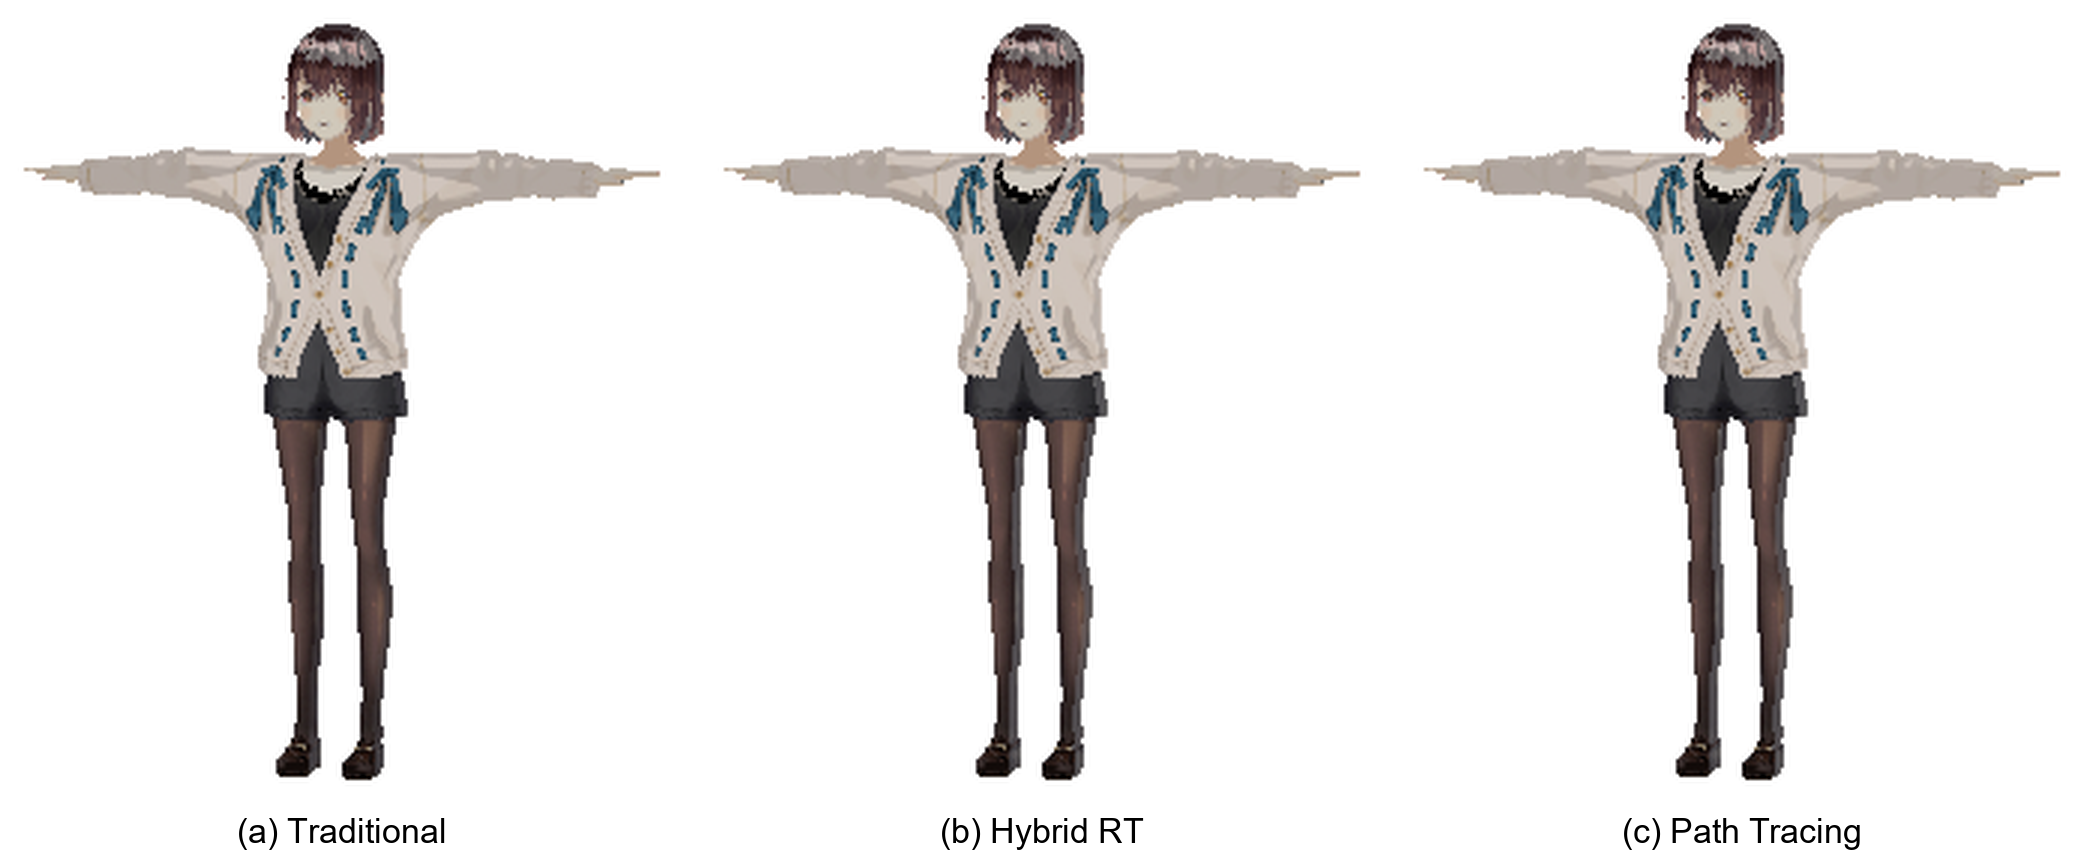
\includegraphics[width=\textwidth]{figures/fig_modes.png}
\caption{The three lighting tiers rendered by the DirectX 12 frame graph at the 640$\times$360 test resolution: (a) Traditional Lighting, (b) Hybrid Ray Tracing, (c) Real-Time 2.5D Path Tracing. Differences are intentionally subtle: all modes share one art direction, and the higher tiers change shadow softness and indirect tint rather than overall appearance.}
\label{fig:modes}
\end{figure*}


\subsection{Indirect Colour Bleeding Before Quantization}
Adding global illumination after the cel step reintroduces the smooth 3D gradients that toon shading exists to remove. AETHER-2.5D instead folds the one-bounce indirect irradiance $E_{ind}$ into the scalar that the quantizer sees. With flat shading normal $N$, key-light direction $L$, ray-traced shadow mask $S$, Rec. 709 luminance $Y(\cdot)$, and bleed strength $k_{gi}$,

\begin{equation}
L_{eff} = (N \cdot L)\,S + k_{gi}\,Y(E_{ind})
\label{eq:leff}
\end{equation}
\begin{equation}
c = \mathrm{smoothstep}(\theta - \phi,\; \theta + \phi,\; L_{eff})
\label{eq:cel}
\end{equation}
where $\theta$ is the material's shadow threshold and $\phi$ a very small feather, so $c$ is effectively binary. A second threshold produces a third, deeper band. The \textit{colour} of the bounce is applied separately, to the shadow albedo only. With $\hat{E} = E_{ind}/\max(E_{ind})$ the normalized bounce chroma and $w = \mathrm{sat}(1.75\,k_{gi}\,Y(E_{ind}))$,

\begin{equation}
A_{sh}' = \mathrm{lerp}\!\left(A_{sh},\; A_{sh} \odot \hat{E},\; w\right)
\label{eq:tint}
\end{equation}
\begin{equation}
C = \mathrm{lerp}\!\left(A_{sh}'\,E_{sh},\; A_{lit}\,E_{lit},\; c\right)
\label{eq:final}
\end{equation}
Bounce light can therefore move a shading boundary and tint a shadow (warm skin colour bleeding onto a white collar, hair colour tinting the forehead), but every boundary remains a single crisp step. Before tinting, shadow colours already receive a hue shift chosen by surface class: skin shifts toward rose, bright neutrals toward periwinkle, and saturated colours toward a deeper, slightly violet tone. Raising $k_{gi}$ from 0 to 1.25 changes the avatar's pixels by a mean of 0.23 RGB levels: a deliberate tint, not a gradient.


\subsection{Dynamic Anisotropic ``Angel Ring''}
Anime hair carries a bright band, the \textit{angel ring}, that follows the head. We reconstruct a crown-to-tip tangent $T$ from screen-space derivatives of position and texture coordinates, project it orthogonal to the normal, and perturb it by a procedural strand-shift curve $s(u)$ and the live SpringBone hair velocity $\mathbf{v}$. Following Scheuermann~\cite{scheuermann}, two shifted tangents produce primary and secondary Kajiya-Kay lobes~\cite{kajiyakay}:

\begin{equation}
T_i = \mathrm{normalize}(T + (s(u) + \delta_i) N + \gamma_i \mathbf{v})
\label{eq:tshift}
\end{equation}
\begin{equation}
\Lambda_i = \left(1 - (T_i \cdot H_i)^2\right)^{\frac{1}{2}\,n_i}
\label{eq:kk}
\end{equation}
where $H_1$ is the half vector of the key light and $H_2$ that of the rim light, so the band responds to both view and lighting. The lobes are passed through a narrow step with a slight chromatic offset between channels, so the ring stays a flat, graphic shape that slides organically when the head tilts. In the test, adding hair velocity changes the upper half of the frame by more than 0.05 RGB levels on average, and a $10^\circ$ camera pitch change moves the ring by more than 2 levels on average.


\subsection{Depth-Offset Rim Light}
A Fresnel term $1 - N\cdot V$ alone draws rims on every curved surface. We combine it with a screen-space test: the shader projects the rim light's direction into screen space, samples linear depth 2--4 pixels toward the light, and treats a relative depth jump $\Delta z / z$ above roughly 0.014--0.048 as a silhouette facing the light. The signal $\max(1 - N\cdot V,\ 0.92\,d_{edge})$ is stepped through a narrow band, multiplied by ray-traced rim occlusion and a light-direction factor, and coloured by the material's rim colour, giving a razor-sharp anime rim whose thickness and position follow the light's azimuth and elevation and the head's motion.


\subsection{2D Filter Pro}
An optional post-process removes the last traces of 3D curvature. A single-pass, four-quadrant Kuwahara filter~\cite{kuwahara} replaces each shaded pixel by the mean of the quadrant with the lowest variance, flattening gradients into painted patches while keeping edges, in the spirit of anisotropic Kuwahara filtering~\cite{kyprianidis}; texture detail such as eyes, lace, and stitching is protected by an edge and ink mask. Ink lines are then strengthened by a flow-guided difference-of-Gaussians on depth and normals~\cite{kang,xdog},

\begin{equation}
D_\sigma(x) = G_\sigma(x) - \tau\,G_{k\sigma}(x)
\label{eq:dog}
\end{equation}
combined with Sobel edges, sub-pixel distance-to-edge anti-aliasing, and depth-aware tapering that keeps silhouettes thick, inner creases thin, and the nose and cheeks clean. An optional paper and cel warmth curve finishes the image. Enabling the filter changes the test frame by a mean of 2.95 RGB levels.

\begin{figure}[!t]
\centering
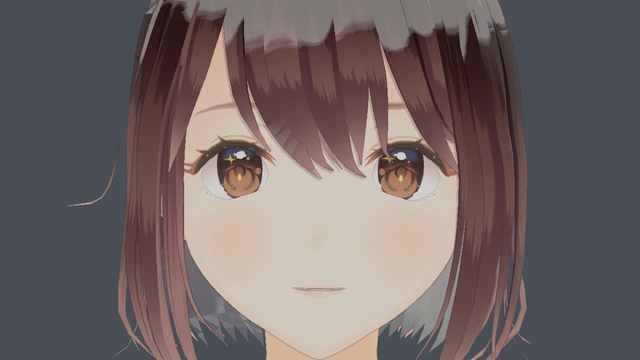
\includegraphics[width=\columnwidth]{figures/fig_face.png}
\caption{Face close-up of the test avatar: SDF face shadow, flattened nose, stepped hair highlight, and coloured ink lines.}
\label{fig:face}
\end{figure}


\subsection{Circadian Lighting}
Streams often run for hours, and lighting that tracks real time of day adds atmosphere. When enabled, the circadian system resolves a clock time from either the system clock or one of 28 fixed UTC offsets from UTC$-$12:00 to UTC+14:00 (for example UTC+07:00 WIB for Jakarta and Surakarta, or UTC+09:00 for Tokyo), or from a manual override between 00:00 and 23:59. It then evaluates a smooth solar trajectory, in the spirit of standard solar-position models~\cite{reda}, and a 24-hour palette for key, fill, and rim intensity, direction, colour temperature~\cite{mccamy}, and shadow hue (Table II). Night never darkens the avatar: it transitions to a ``Night Studio'' of moonlight rim and monitor-glow key. The tests confirm the two-hour difference between UTC+07:00 and UTC+09:00, the phase classification, a golden-hour key below 3800 K, a daytime key above 5200 K, night key intensity of at least 1.0, and continuity across midnight.

\begin{table}[!t]
\renewcommand{\arraystretch}{1.15}
\caption{Circadian lighting palette}
\label{tab:circadian}
\centering\footnotesize
\begin{tabular}{p{0.188\columnwidth}p{0.207\columnwidth}p{0.188\columnwidth}p{0.357\columnwidth}}
\hline
\textbf{Phase} & \textbf{Hours} & \textbf{Key light} & \textbf{Character} \\
\hline
Dawn & 05:00--07:00 & $\sim$3600 K & Low east sun, rose-peach key, periwinkle fill \\
Day & 07:00--15:30 & $\sim$5800 K & High clean daylight, sky-blue fill \\
Golden hour & 15:30--18:00 & $\sim$3100 K & Low west sun, amber key, violet shadows, warm rim \\
Night Studio & 18:00--05:00 & $\sim$4600 K & Silver moon rim ($\sim$6500 K), cyan/lavender monitor key, warm fill \\
\hline
\end{tabular}
\end{table}


\section{Output and Integration}
T4 publishes each completed frame without a CPU round trip where possible. Spout2~\cite{spout} receives a shared Direct3D 11 texture created from the same GPU (matched by adapter LUID), imported into Vulkan via \texttt{VK\_\allowbreak{}KHR\_\allowbreak{}external\_\allowbreak{}memory\_\allowbreak{}win32}, or shared from DirectX 12 through D3D11On12; publishing costs 0.185 ms. A dependency-free DirectShow filter, built for both x64 and x86 hosts, exposes a virtual webcam in ARGB32, RGB32, or NV12 at 1080p or 720p and 60 or 30 fps, reading frames from a triple-buffered shared-memory region protected by a seqlock; the copy takes 0.483 ms at the 95th percentile. An NDI 6 sender~\cite{ndi} is loaded dynamically when the runtime is installed. The studio also sends OSC and VMC telemetry, and accepts an opt-in, bearer-token-authenticated WebSocket control channel. Plugins run either as typed node graphs compiled by the Rust host or as WebAssembly components~\cite{wasm} in wasmtime~\cite{wasmtime} with a 64 MiB memory limit and 2 ms execution deadlines.


\section{Implementation and Verification}
The code base comprises approximately 54,000 lines of C++ in 180 files, 20,900 lines of Rust in 47 files, 2,000 lines of Slang in 14 shader files, and 11,800 lines of tests in 34 files. Four CMake presets build Debug (validation layers and the allocation guard), RelWithDebInfo (with the Tracy profiler), Release (link-time optimization), and a CI configuration with AddressSanitizer and GPU-assisted validation. All presets compile with \texttt{/W4 /WX}; the Rust workspace passes \texttt{cargo clippy -D warnings} and \texttt{cargo deny} licence checks; Vulkan validation and the D3D12 debug layer must report zero errors.

Thirty Catch2 suites verify the system. They range from FFI layout and lock-free container tests, through tracking latency, filter, IK, and SIMD SpringBone tests, to GPU tests that render a real VRM avatar headlessly: FLIP golden images across six scenes with ray tracing on and off, cross-vendor parity, denoiser budgets, device-lost recovery, Spout2 and virtual-camera transport, motion-to-photon latency, DirectX 11 and 12 parity, and UI frame budgets with PNG snapshots. Every number in Section IX is printed by these tests.


\section{Results}
Table III summarizes measured performance on a laptop with an NVIDIA GeForce RTX 5060 Laptop GPU and an Intel Core Ultra processor with an AI Boost NPU, at 1080p unless noted, in RelWithDebInfo builds. Budgets are those of the specification.

\begin{table}[!t]
\renewcommand{\arraystretch}{1.15}
\caption{Measured performance (95th percentile unless noted)}
\label{tab:perf}
\centering\footnotesize
\begin{tabular}{p{0.526\columnwidth}p{0.188\columnwidth}p{0.226\columnwidth}}
\hline
\textbf{Measurement} & \textbf{Budget} & \textbf{Measured} \\
\hline
NPU face landmarks + blendshapes & $\le$ 6.0 ms & 3.35 ms \\
NPU body + face + blendshapes & $\le$ 12.0 ms & 7.44 ms \\
iGPU tracking fallback & $\le$ 35 ms & 8.58 ms \\
AVX2 ROI pre-processing & $\le$ 0.60 ms & 0.24 ms \\
SimEngine tick, 512 springs & $\le$ 0.80 ms & 0.052 ms \\
RT critical path, passes 1--12 & $\le$ 4.2 ms & 2.67 ms \\
Denoiser & $\le$ 0.80 ms & 0.56 ms \\
Motion-to-photon, RT on & --- & 8.33 ms \\
Spout2 publish & --- & 0.185 ms \\
Virtual-camera copy & --- & 0.483 ms \\
Studio UI, 64-node graph & $\le$ 0.40 ms & 0.143 ms \\
Device-lost recovery & $\le$ 3000 ms & 260 ms \\
\hline
\end{tabular}
\end{table}

\begin{table}[!t]
\renewcommand{\arraystretch}{1.15}
\caption{Image-quality and correctness checks}
\label{tab:quality}
\centering\footnotesize
\begin{tabular}{p{0.451\columnwidth}p{0.226\columnwidth}p{0.263\columnwidth}}
\hline
\textbf{Check} & \textbf{Criterion} & \textbf{Result} \\
\hline
DX12 vs Vulkan IoU (upright) & $\ge$ 0.85 & 1.000 \\
DX12 vs flipped / mirrored & lower & 0.380 / 0.880 \\
DX12 vs Vulkan RGB diff & < 25 & 0.45 \\
Golden images, 12 scenes (FLIP) & $\le$ 0.05 & 0.0000 \\
RTX 5060 vs Intel Xe (FLIP) & $\le$ 0.05 & 0.00084--0.00267 \\
PT stillness (RGB diff) & < 2.0 & 0.0105 \\
Bloom white composite $\Delta$E & $\le$ 1.0 & 0.332 \\
Anti-clip residual (2,145 pts) & = 0 & 0.000 m \\
Nose foreshortening reduction & $\ge$ 70 \% & 73.6 \% \\
\hline
\end{tabular}
\end{table}

All budgets are met with margin. The ray-traced critical path uses 64 \% of its 4.2 ms budget, leaving room for the path-tracing tier at 60 FPS; motion-to-photon latency of 8.33 ms is below one 60 Hz frame. The orientation and anti-clipping checks hold exactly rather than approximately. Image-quality results show that stylization and robustness features do not trade away correctness: golden images are bit-stable, and different GPU vendors produce near-identical frames.


\section{Discussion and Limitations}
The engine targets Windows only, because its outputs (DirectShow, Spout2, D3D11 interop) and NPU routing depend on Windows APIs. All performance figures come from a single laptop; integrated-GPU results are limited to correctness and the absence of device loss, not a full timing study. The rendering tests use one VRM avatar, and stylization quality is ultimately an aesthetic judgement that pixel metrics capture only partly. The anti-clipping model uses fixed capsule proportions derived from a canonical humanoid rather than fitting capsules to each avatar, and the circadian model is an artistic palette over a solar trajectory, not a radiometric sky model. NDI output requires a separately installed runtime. Finally, the path-tracing tier trades a small amount of temporal responsiveness for stillness; under very fast motion, history clamping falls back to the spatial filter.


\section{Conclusion}
AETHER-2.5D Studio shows that a VTuber engine can combine NPU-accelerated tracking, three graphics APIs, and three lighting tiers from rasterization to path tracing without sacrificing either latency or a flat, hand-drawn look. The key design decisions are to enforce physical plausibility in the tracking stage before animation, to make coordinate conventions an explicitly tested contract across APIs, and to feed physically based light into the cel quantizer rather than on top of it. Future work includes per-avatar collision fitting, a wider hardware study, and user studies of perceived stylization quality.


\section*{Availability and License}
AETHER-2.5D Studio is source-available under the AETHER-2.5D Studio Source-Available, No-Derivatives, No-AI License v1.0. The software may not be modified, redistributed, re-implemented, or used to train or evaluate machine-learning systems. Contributions are welcome after contacting the author at ramzyhaidar20@gmail.com.

\section*{Acknowledgment}
The author thanks the developers of MediaPipe, ONNX Runtime, OpenVINO, Slang, Dear ImGui, and the VRM Consortium, whose openly licensed work this system builds on.

\begin{thebibliography}{55}
\bibitem{live2d} Live2D Inc., ``Live2D Cubism,'' 2024. [Online]. Available: \url{https://www.live2d.com/en/}
\bibitem{vrm} VRM Consortium, ``VRM 1.0 specification,'' 2022. [Online]. Available: \url{https://github.com/vrm-c/vrm-specification}
\bibitem{mediapipe} C. Lugaresi \textit{et al.}, ``MediaPipe: A framework for building perception pipelines,'' arXiv:1906.08172, 2019.
\bibitem{blazeface} V. Bazarevsky, Y. Kartynnik, A. Vakunov, K. Raveendran, and M. Grundmann, ``BlazeFace: Sub-millisecond neural face detection on mobile GPUs,'' arXiv:1907.05047, 2019.
\bibitem{facemesh} Y. Kartynnik, A. Ablavatski, I. Grishchenko, and M. Grundmann, ``Real-time facial surface geometry from monocular video on mobile GPUs,'' arXiv:1907.06724, 2019.
\bibitem{blazepose} V. Bazarevsky, I. Grishchenko, K. Raveendran, T. Zhu, F. Zhang, and M. Grundmann, ``BlazePose: On-device real-time body pose tracking,'' arXiv:2006.10204, 2020.
\bibitem{mphands} F. Zhang \textit{et al.}, ``MediaPipe Hands: On-device real-time hand tracking,'' arXiv:2006.10214, 2020.
\bibitem{gower} J. C. Gower, ``Generalized Procrustes analysis,'' \textit{Psychometrika}, vol. 40, no. 1, pp. 33--51, 1975.
\bibitem{kabsch} W. Kabsch, ``A solution for the best rotation to relate two sets of vectors,'' \textit{Acta Crystallographica Section A}, vol. 32, no. 5, pp. 922--923, 1976.
\bibitem{oneeuro} G. Casiez, N. Roussel, and D. Vogel, ``1\texteuro{} filter: A simple speed-based low-pass filter for noisy input in interactive systems,'' in \textit{Proc. ACM CHI Conf. Human Factors in Computing Systems}, 2012, pp. 2527--2530.
\bibitem{kalman} R. E. Kalman, ``A new approach to linear filtering and prediction problems,'' \textit{Journal of Basic Engineering}, vol. 82, no. 1, pp. 35--45, 1960.
\bibitem{lake} A. Lake, C. Marshall, M. Harris, and M. Blackstein, ``Stylized rendering techniques for scalable real-time 3D animation,'' in \textit{Proc. 1st Int. Symp. Non-Photorealistic Animation and Rendering (NPAR)}, 2000, pp. 13--20.
\bibitem{gooch98} A. Gooch, B. Gooch, P. Shirley, and E. Cohen, ``A non-photorealistic lighting model for automatic technical illustration,'' in \textit{Proc. SIGGRAPH}, 1998, pp. 447--452.
\bibitem{npr_book} B. Gooch and A. Gooch, \textit{Non-Photorealistic Rendering}. Natick, MA, USA: A K Peters, 2001.
\bibitem{raskar} R. Raskar and M. Cohen, ``Image precision silhouette edges,'' in \textit{Proc. ACM Symp. Interactive 3D Graphics (I3D)}, 1999, pp. 135--140.
\bibitem{ggxrd} J. Motomura, ``GuiltyGearXrd's art style: The X factor between 2D and 3D,'' presented at the Game Developers Conf. (GDC), San Francisco, CA, USA, 2015.
\bibitem{mtoon} Santarh, ``MToon,'' GitHub repository, 2018. [Online]. Available: \url{https://github.com/Santarh/MToon}
\bibitem{kajiya86} J. T. Kajiya, ``The rendering equation,'' \textit{ACM SIGGRAPH Computer Graphics}, vol. 20, no. 4, pp. 143--150, 1986.
\bibitem{pbrt} M. Pharr, W. Jakob, and G. Humphreys, \textit{Physically Based Rendering: From Theory to Implementation}, 3rd ed. Cambridge, MA, USA: Morgan Kaufmann, 2016.
\bibitem{dxr} Microsoft, ``DirectX Raytracing (DXR) functional spec,'' 2023. [Online]. Available: \url{https://microsoft.github.io/DirectX-Specs/d3d/Raytracing.html}
\bibitem{vulkan} The Khronos Group, ``Vulkan 1.3 specification (with KHR extensions),'' 2022. [Online]. Available: \url{https://registry.khronos.org/vulkan/}
\bibitem{svgf} C. Schied \textit{et al.}, ``Spatiotemporal variance-guided filtering: Real-time reconstruction for path-traced global illumination,'' in \textit{Proc. High Performance Graphics (HPG)}, 2017, pp. 2:1--2:12.
\bibitem{karis} B. Karis, ``High-quality temporal supersampling,'' in \textit{Advances in Real-Time Rendering in Games, ACM SIGGRAPH Courses}, 2014.
\bibitem{wachter} C. Wächter and N. Binder, ``A fast and robust method for avoiding self-intersection,'' in \textit{Ray Tracing Gems}, E. Haines and T. Akenine-Möller, Eds. Berkeley, CA, USA: Apress, 2019, pp. 77--85.
\bibitem{pcss} R. Fernando, ``Percentage-closer soft shadows,'' in \textit{ACM SIGGRAPH Sketches}, 2005, p. 35.
\bibitem{heitz} E. Heitz, L. Belcour, V. Ostromoukhov, D. Coeurjolly, and J.-C. Iehl, ``A low-discrepancy sampler that distributes Monte Carlo errors as a blue noise in screen space,'' in \textit{ACM SIGGRAPH Talks}, 2019, pp. 68:1--68:2.
\bibitem{kuwahara} M. Kuwahara, K. Hachimura, S. Eiho, and M. Kinoshita, ``Processing of RI-angiocardiographic images,'' in \textit{Digital Processing of Biomedical Images}, K. Preston and M. Onoe, Eds. New York, NY, USA: Plenum Press, 1976, pp. 187--202.
\bibitem{kyprianidis} J. E. Kyprianidis, H. Kang, and J. Döllner, ``Image and video abstraction by anisotropic Kuwahara filtering,'' \textit{Computer Graphics Forum}, vol. 28, no. 7, pp. 1955--1963, 2009.
\bibitem{tomasi} C. Tomasi and R. Manduchi, ``Bilateral filtering for gray and color images,'' in \textit{Proc. IEEE Int. Conf. Computer Vision (ICCV)}, 1998, pp. 839--846.
\bibitem{kang} H. Kang, S. Lee, and C. K. Chui, ``Coherent line drawing,'' in \textit{Proc. 5th Int. Symp. Non-Photorealistic Animation and Rendering (NPAR)}, 2007, pp. 43--50.
\bibitem{xdog} H. Winnemöller, J. E. Kyprianidis, and S. C. Olsen, ``XDoG: An eXtended difference-of-Gaussians compendium including advanced image stylization,'' \textit{Computers \& Graphics}, vol. 36, no. 6, pp. 740--753, 2012.
\bibitem{kajiyakay} J. T. Kajiya and T. L. Kay, ``Rendering fur with three dimensional textures,'' \textit{ACM SIGGRAPH Computer Graphics}, vol. 23, no. 3, pp. 271--280, 1989.
\bibitem{marschner} S. R. Marschner, H. W. Jensen, M. Cammarano, S. Worley, and P. Hanrahan, ``Light scattering from human hair fibers,'' \textit{ACM Trans. Graphics}, vol. 22, no. 3, pp. 780--791, 2003.
\bibitem{scheuermann} T. Scheuermann, ``Practical real-time hair rendering and shading,'' in \textit{ACM SIGGRAPH Sketches}, 2004, p. 147.
\bibitem{herlihy} M. Herlihy and N. Shavit, \textit{The Art of Multiprocessor Programming}. Burlington, MA, USA: Morgan Kaufmann, 2008.
\bibitem{gltf} The Khronos Group, ``glTF 2.0 specification,'' 2021. [Online]. Available: \url{https://registry.khronos.org/glTF/}
\bibitem{wasm} A. Haas \textit{et al.}, ``Bringing the web up to speed with WebAssembly,'' in \textit{Proc. 38th ACM SIGPLAN Conf. Programming Language Design and Implementation (PLDI)}, 2017, pp. 185--200.
\bibitem{wasmtime} Bytecode Alliance, ``Wasmtime: A fast and secure runtime for WebAssembly,'' 2025. [Online]. Available: \url{https://wasmtime.dev}
\bibitem{fraser} K. Fraser, ``Practical lock-freedom,'' Ph.D. dissertation, Computer Laboratory, Univ. Cambridge, Cambridge, U.K., Tech. Rep. UCAM-CL-TR-579, 2004.
\bibitem{dijkstra} E. W. Dijkstra, L. Lamport, A. J. Martin, C. S. Scholten, and E. F. M. Steffens, ``On-the-fly garbage collection: An exercise in cooperation,'' \textit{Communications of the ACM}, vol. 21, no. 11, pp. 966--975, 1978.
\bibitem{arkit} Apple Inc., ``ARFaceAnchor.BlendShapeLocation,'' Apple Developer Documentation, 2024. [Online]. Available: \url{https://developer.apple.com/documentation/arkit/arfaceanchor/blendshapelocation}
\bibitem{ort} ONNX Runtime developers, ``ONNX Runtime,'' Microsoft, 2021. [Online]. Available: \url{https://onnxruntime.ai}
\bibitem{openvino} Intel Corporation, ``OpenVINO toolkit documentation,'' 2025. [Online]. Available: \url{https://docs.openvino.ai}
\bibitem{ericson} C. Ericson, \textit{Real-Time Collision Detection}. San Francisco, CA, USA: Morgan Kaufmann, 2005.
\bibitem{pbd} M. Müller, B. Heidelberger, M. Hennix, and J. Ratcliff, ``Position based dynamics,'' \textit{Journal of Visual Communication and Image Representation}, vol. 18, no. 2, pp. 109--118, 2007.
\bibitem{fabrik} A. Aristidou and J. Lasenby, ``FABRIK: A fast, iterative solver for the inverse kinematics problem,'' \textit{Graphical Models}, vol. 73, no. 5, pp. 243--260, 2011.
\bibitem{jakobsen} T. Jakobsen, ``Advanced character physics,'' in \textit{Proc. Game Developers Conf. (GDC)}, San Jose, CA, USA, 2001.
\bibitem{slang} Y. He, K. Fatahalian, and T. Foley, ``Slang: Language mechanisms for extensible real-time shading systems,'' \textit{ACM Trans. Graphics}, vol. 37, no. 4, pp. 141:1--141:13, 2018.
\bibitem{bjorge} M. Bjørge, ``Bandwidth-efficient rendering,'' in \textit{Moving Mobile Graphics, ACM SIGGRAPH Courses}, 2015.
\bibitem{spout} L. Jarvis, ``Spout: Realtime video sharing for Windows,'' 2024. [Online]. Available: \url{https://spout.zeal.co}
\bibitem{flip} P. Andersson, J. Nilsson, T. Akenine-Möller, M. Oskarsson, K. Åström, and M. D. Fairchild, ``FLIP: A difference evaluator for alternating images,'' \textit{Proc. ACM Computer Graphics and Interactive Techniques}, vol. 3, no. 2, pp. 15:1--15:23, 2020.
\bibitem{ramamoorthi} R. Ramamoorthi and P. Hanrahan, ``An efficient representation for irradiance environment maps,'' in \textit{Proc. SIGGRAPH}, 2001, pp. 497--500.
\bibitem{reda} I. Reda and A. Andreas, ``Solar position algorithm for solar radiation applications,'' \textit{Solar Energy}, vol. 76, no. 5, pp. 577--589, 2004.
\bibitem{mccamy} C. S. McCamy, ``Correlated color temperature as an explicit function of chromaticity coordinates,'' \textit{Color Research \& Application}, vol. 17, no. 2, pp. 142--144, 1992.
\bibitem{ndi} Vizrt NDI AB, ``NDI 6 SDK documentation,'' 2024. [Online]. Available: \url{https://docs.ndi.video}
\end{thebibliography}

\end{document}
